\section{Comunidade acadêmica}
\label{s.community}

\begin{frame}{Comunidade acadêmica}
	\justify 
	\begin{itemize}
		\item<1> Grupo de pessoas de instituições de ensino superior as quais engajam-se em atividades ``intelectuais", tais como ensino, aprendizado e pesquisa;
		\\~\\
		\item<2> Comunidade deve ser inclusiva, diversa e abrangente, não limitando a participação de quaisquer pessoas;
		\\~\\
		\item<3> Como garantir que as pesquisas sejam ``honestas"~e sigam um conjunto de boas práticas?
	\end{itemize}
\end{frame}

\begin{frame}{}
	\centering
	\begin{figure}
		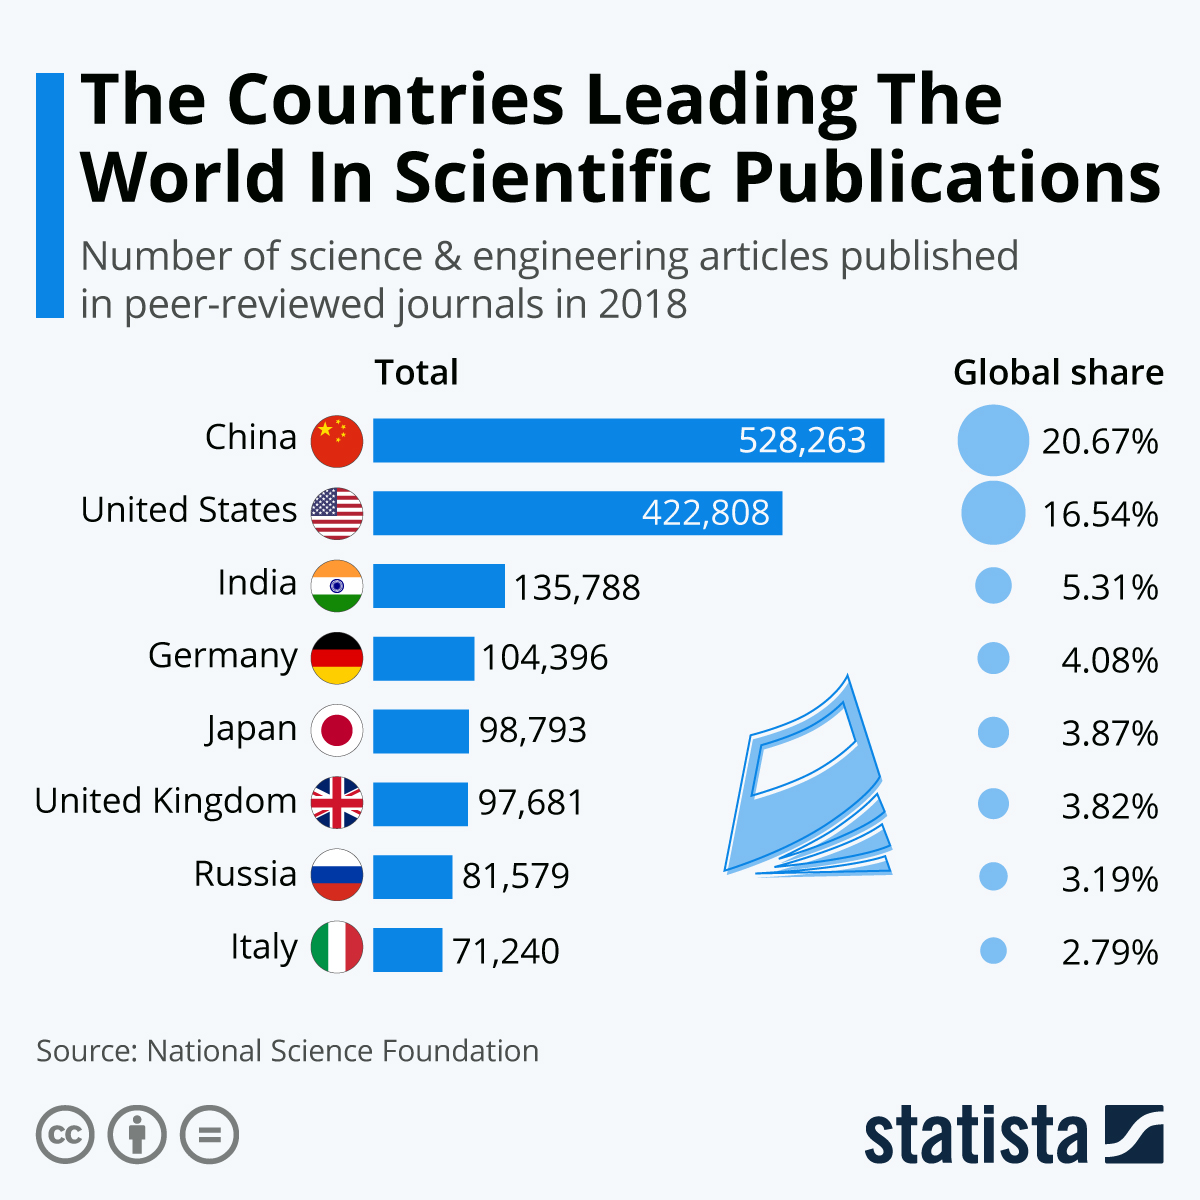
\includegraphics[scale=0.125]{figs/lead_country_papers.png}
		\caption{Ranking de países líderes em publicações nas áreas de Ciência e Engenharia no ano de 2018~\cite{Statista:18}.}
		\label{f.lead_country_papers}
	\end{figure}
\end{frame}

\subsection{Reprodutibilidade e integridade}
\label{ss.reproducibility_integrity}

\begin{frame}{Reprodutibilidade e integridade}
\end{frame}

\subsection{Impacto social}
\label{ss.social_impact}

\begin{frame}{Impacto social}
\end{frame}
